\documentclass[notes,11pt, aspectratio=169]{beamer}

\usepackage{pgfpages}
% These slides also contain speaker notes. You can print just the slides,
% just the notes, or both, depending on the setting below. Comment out the want
% you want.
\setbeameroption{hide notes} % Only slide
%\setbeameroption{show only notes} % Only notes
%\setbeameroption{show notes on second screen=right} % Both

\usepackage{helvet}
\usepackage[default]{lato}
\usepackage{array}
\usepackage{tgbonum}

\usepackage{tikz}
\usepackage{verbatim}
\setbeamertemplate{note page}{\pagecolor{yellow!5}\insertnote}
\usetikzlibrary{positioning}
\usetikzlibrary{snakes}
\usetikzlibrary{calc}
\usetikzlibrary{arrows}
\usetikzlibrary{decorations.markings}
\usetikzlibrary{shapes.misc}
\usetikzlibrary{matrix,shapes,arrows,fit,tikzmark}
\usepackage{amsmath}
\usepackage{mathpazo}
\usepackage{hyperref}
\usepackage{lipsum}
\usepackage{multimedia}
\usepackage{graphicx}
\usepackage{multirow}
\usepackage{graphicx}
\usepackage{dcolumn}
\usepackage{bbm}
\newcolumntype{d}[0]{D{.}{.}{5}}

\usepackage{changepage}
\usepackage{appendixnumberbeamer}
\newcommand{\beginbackup}{
   \newcounter{framenumbervorappendix}
   \setcounter{framenumbervorappendix}{\value{framenumber}}
   \setbeamertemplate{footline}
   {
     \leavevmode%
     \hline
     box{%
       \begin{beamercolorbox}[wd=\paperwidth,ht=2.25ex,dp=1ex,right]{footlinecolor}%
%         \insertframenumber  \hspace*{2ex} 
       \end{beamercolorbox}}%
     \vskip0pt%
   }
 }
\newcommand{\backupend}{
   \addtocounter{framenumbervorappendix}{-\value{framenumber}}
   \addtocounter{framenumber}{\value{framenumbervorappendix}} 
}


\usepackage{graphicx}
\usepackage[space]{grffile}
\usepackage{booktabs}
\newcommand\independent{\protect\mathpalette{\protect\independenT}{\perp}}
\def\independenT#1#2{\mathrel{\rlap{$#1#2$}\mkern2mu{#1#2}}}
\DeclareMathOperator{\Supp}{Supp}

% These are my colors -- there are many like them, but these ones are mine.
\definecolor{blue}{RGB}{0,114,178}
\definecolor{red}{RGB}{213,94,0}
\definecolor{yellow}{RGB}{240,228,66}
\definecolor{green}{RGB}{0,158,115}

\hypersetup{
  colorlinks=false,
  linkbordercolor = {white},
  linkcolor = {blue}
}


%% I use a beige off white for my background
\definecolor{MyBackground}{RGB}{255,253,218}

%% Uncomment this if you want to change the background color to something else
%\setbeamercolor{background canvas}{bg=MyBackground}

%% Change the bg color to adjust your transition slide background color!
\newenvironment{transitionframe}{
  \setbeamercolor{background canvas}{bg=yellow}
  \begin{frame}}{
    \end{frame}
}

\setbeamercolor{frametitle}{fg=blue}
\setbeamercolor{title}{fg=black}
\setbeamertemplate{footline}[frame number]
\setbeamertemplate{navigation symbols}{} 
\setbeamertemplate{itemize items}{-}
\setbeamercolor{itemize item}{fg=blue}
\setbeamercolor{itemize subitem}{fg=blue}
\setbeamercolor{enumerate item}{fg=blue}
\setbeamercolor{enumerate subitem}{fg=blue}
\setbeamercolor{button}{bg=MyBackground,fg=blue,}



% If you like road maps, rather than having clutter at the top, have a roadmap show up at the end of each section 
% (and after your introduction)
% Uncomment this is if you want the roadmap!
% \AtBeginSection[]
% {
%    \begin{frame}
%        \frametitle{Roadmap of Talk}
%        \tableofcontents[currentsection]
%    \end{frame}
% }
\setbeamercolor{section in toc}{fg=blue}
\setbeamercolor{subsection in toc}{fg=red}
\setbeamersize{text margin left=1em,text margin right=1em} 

\newenvironment{wideitemize}{\itemize\addtolength{\itemsep}{10pt}}{\enditemize}

\usepackage{environ}
\NewEnviron{videoframe}[1]{
  \begin{frame}
    \vspace{-8pt}
    \begin{columns}[onlytextwidth, T] % align columns
      \begin{column}{.70\textwidth}
        \begin{minipage}[t][\textheight][t]
          {\dimexpr\textwidth}
          \vspace{8pt}
          \hspace{4pt} {\Large \sc \textcolor{blue}{#1}}
          \vspace{8pt}
          
          \BODY
        \end{minipage}
      \end{column}%
      \hfill%
      \begin{column}{.38\textwidth}
        \colorbox{green!20}{\begin{minipage}[t][1.2\textheight][t]
            {\dimexpr\textwidth}
            Face goes here
          \end{minipage}}
      \end{column}%
    \end{columns}
  \end{frame}
}

\title[]{\textcolor{blue}{Canonical Research Designs IV:\\ Instrumental Variables II }}
\author[PGP]{}
\institute[FRBNY]{\small{\begin{tabular}{c}
  Paul Goldsmith-Pinkham  \\
\end{tabular}}}

\date{\today}

\begin{document}

%%% TIKZ STUFF
\tikzset{   
        every picture/.style={remember picture,baseline},
        every node/.style={anchor=base,align=center,outer sep=1.5pt},
        every path/.style={thick},
        }
\newcommand\marktopleft[1]{%
    \tikz[overlay,remember picture] 
        \node (marker-#1-a) at (-.3em,.3em) {};%
}
\newcommand\markbottomright[2]{%
    \tikz[overlay,remember picture] 
        \node (marker-#1-b) at (0em,0em) {};%
}
\tikzstyle{every picture}+=[remember picture] 
\tikzstyle{mybox} =[draw=black, very thick, rectangle, inner sep=10pt, inner ysep=20pt]
\tikzstyle{fancytitle} =[draw=black,fill=red, text=white]
%%%% END TIKZ STUFF

% Title Slide
\begin{frame}
\maketitle
\end{frame}

\begin{frame}{Roadmap for Today}
    \begin{enumerate}
    \item Reiterating why it's easy to screw up exclusion. Discuss two examples:
      \begin{itemize}
      \item lottery
      \item weather
      \end{itemize}
    \item Marginal treatment effects
    \item Discuss why better LATE than never      
    \item How monotonicity can fail
    \item Characterizing compliers
    \end{enumerate}

\end{frame}

%    \item Next class: (estimation) overid bias (jackknife)
%    \item Next class: (estimation) weak iv bias (pre-test)
%    \item Next class: (estimation) IVQTE
%    \item Next class: (estimation) Lasso IV

\begin{frame}{Why is the exclusion restriction challenging?}
  \begin{columns}[T] % align columns
    \begin{column}{0.6\textwidth}
      \begin{wideitemize}
      \item Recall the key (untestable) feature for IV: exclusion
        restriction
      \item In the context of the DAG, the intuition is that $Z$ only
        affects $Y$ through $D$
      \item Intuitively, it feels like something randomly assigned or
        nearly random should satisfy this, so long as it affects $D$
      \item \emph{This is not sufficient }
        \begin{itemize}
        \item You need to think critically about the IV
        \end{itemize}
  \end{wideitemize}
\end{column}
\begin{column}{0.4\textwidth}
  \begin{center}
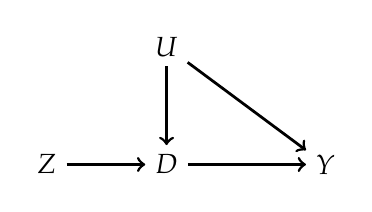
\begin{tikzpicture}
        % nodes %
        % \node[text centered] (z) {$Z$};
        \node[text centered] (t) {$D$};
        \node[right=1.5 of t, text centered] (y) {$Y$};
        \node[above = 1 of t, text centered] (u) {$U$};
        \node[left = 1 of t, text centered] (z) {$Z$};        
        % edges %
        \draw[->, line width= 1] (z) --  (t);
        \draw [->, line width= 1] (t) -- (y);
        % \draw[->,red, line width= 1,dashed] (u) --node {X} (z);
        \draw[->,line width= 1] (u) --(t);
%        \draw[->,line width= 1] (z) --(t);
 %       \draw[->,bend right, line width= 1] (z) to [out=-50,in=-130]  (y);                
        \draw[->,line width= 1] (u) -- (y);
%\draw[->, red, line width=1,dashed] (z) to  [out=270,in=270, looseness=0.5] node{X} (y);
      \end{tikzpicture}
      \end{center}
\end{column}
\end{columns}
\end{frame}


\begin{frame}{Why is the exclusion restriction challenging?}
  \begin{columns}[T] % align columns
    \begin{column}{0.6\textwidth}
      \begin{wideitemize}
      \item Consider two examples. First, using Vietnam war lottery
        numbers as an IV for military service, studying the impact on
        mortality.
        \begin{itemize}
        \item $Y$: death, $D$: vietnam vet, $Z$: lottery number
        \end{itemize}
      \item Lottery number was randomly assigned as a function of birthdate
        \begin{itemize}
        \item Well-defined design-based view of $Z$ allocation! 
        \end{itemize}
      \item Does that necessarily satisfy exclusion restriction? Seems
        like a pretty slam dunk IV
        \begin{itemize}
        \item Clearly affects veteran status
        \item Clearly random!
        \end{itemize}
  \end{wideitemize}
\end{column}
\begin{column}{0.4\textwidth}
  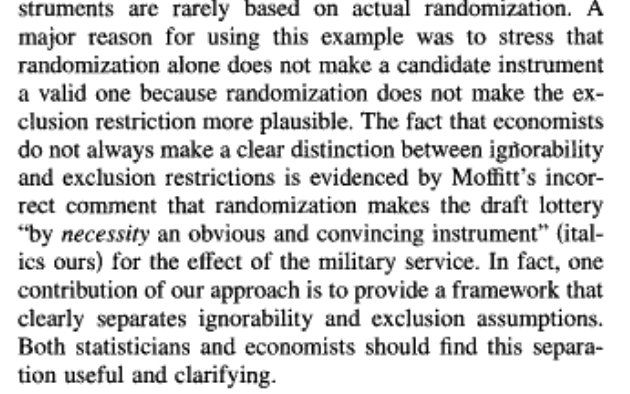
\includegraphics[width=\linewidth]{images/jasaa.png}
\end{column}
\end{columns}
\end{frame}


\begin{frame}{Why is the exclusion restriction challenging?}
  \begin{columns}[T] % align columns
    \begin{column}{0.6\textwidth}
      \begin{wideitemize}
      \item Does that necessarily satisfy exclusion restriction? 
        \begin{itemize}
        \item Not necessarily!
        \end{itemize}
      \item Why? Consider one simple example: being drafted induces
        you to change your behavior to \emph{avoid} the draft
        \begin{itemize}
        \item Stay in school
        \item Flee to Canada
        \end{itemize}
      \item This would violate the exclusion restriction!
  \end{wideitemize}
\end{column}
\begin{column}{0.4\textwidth}
  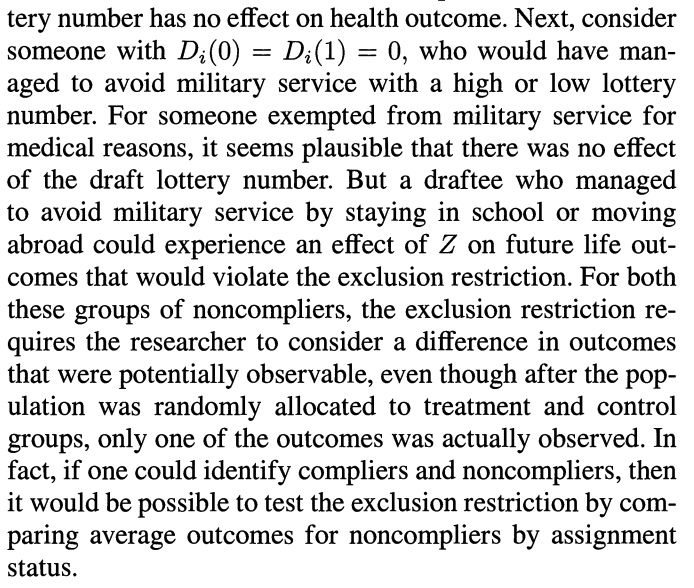
\includegraphics[width=\linewidth]{images/jasab.png}
\end{column}
\end{columns}
\end{frame}


\begin{frame}{Why is the exclusion restriction challenging?}
  \begin{columns}[T] % align columns
    \begin{column}{0.6\textwidth}
      \begin{wideitemize}
      \item Second, consider rainfall as an instrument for income in
        agriculture environments (many crops are heavily dependent on
        it)
        \begin{itemize}
        \item This is not uncommon in development papers, as Sarsons
          (2015) points out
        \item $Y$: conflict, $D$: income, $Z$: rainfall
        \end{itemize}
      \item Exclusion restriction is that rainfall has no effect on
        conflict \emph{beyond} income
        \begin{itemize}
        \item While the logic seems reasonable, Sarsons (2015) shows
          that places with dams (which protect against the income shocks
          due to rain) have similar conflict to those without dams
        \end{itemize}
      \item Plausible that while rain is ``\emph{random}'', it might
        have many channels
      \end{wideitemize}
\end{column}
\begin{column}{0.4\textwidth}
  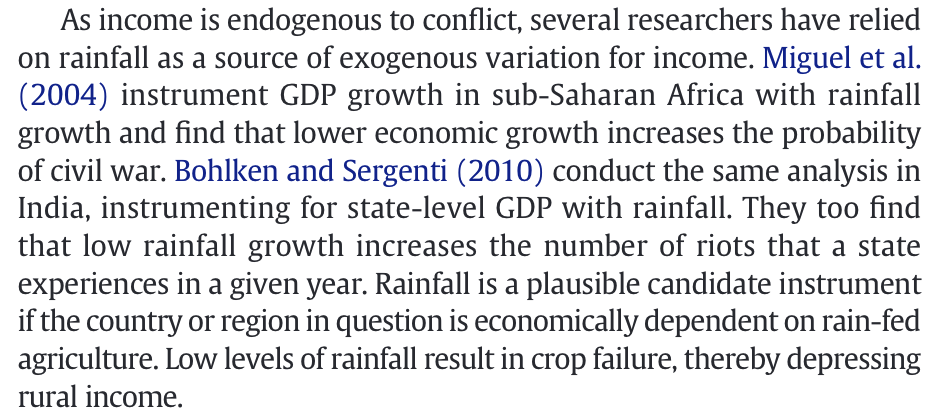
\includegraphics[width=\linewidth]{images/sarsonsa.png}\\
      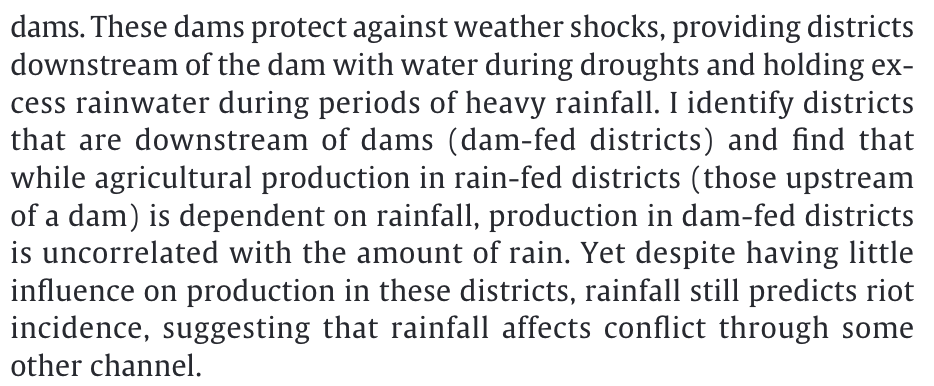
\includegraphics[width=\linewidth]{images/sarsonsb.png}\\
\end{column}
\end{columns}
\end{frame}

\begin{frame}{Exclusion Restrictions}
  \begin{columns}[T] % align columns
    \begin{column}{0.85\textwidth}
      \begin{wideitemize}
      \item Even with a variable that is near-random in its
        allocation, the exclusion restriction is not always satisfied
        \begin{itemize}
        \item Worse yet, it's a fundamentally untestable restriction
        \end{itemize}
      \item Using an IV requires thinking carefully about justifying
        the exclusion restriction
        \begin{itemize}
      \item It can also be useful to think about what
          violations in the restriction implies
        \end{itemize}
      \item $Y_{i} = Y_{i}(Z_{i}, D_{i}(Z_{i}))$. Let
        $H_{i} = Y_{i}(1,d) - Y_{i}(0,d)$, where $d$ is 1 for an
        always-taker, and $d$ is 0 for a never-taker.
        \begin{itemize}
      \item Under monotonicity, (Angrist, Imbens, and Rubin (1996)):
        \end{itemize}
          \begin{align*}
            \frac{E(Y_{i}(1, D_{i}(1)) - Y_{i}(0, D_{i}(0)))}{E(D_{i}(1) - D_{i}(0))} &= E(Y_{i}(1, D_{i}(1)) -  Y_{i}(0, D_{i}(0)) | \text{$i$ is a complier})\\
            &+ E(H_{i} | \text{$i$ is a noncomplier}) \cdot \frac{\Pr(\text{$i$ is a noncomplier})}{Pr(\text{$i$ is a complier})}
          \end{align*}
      \end{wideitemize}
\end{column}
\begin{column}{0.4\textwidth}
\end{column}
\end{columns}
\end{frame}

\begin{frame}{Knowable things about Exclusion Restriction violations}
  \begin{columns}[T] % align columns
    \begin{column}{0.99\textwidth}
          \begin{align*}
            \frac{E(Y_{i}(1, D_{i}(1)) - Y_{i}(0, D_{i}(0)))}{E(D_{i}(1) - D_{i}(0))} &= E(Y_{i}(1, D_{i}(1)) -  Y_{i}(0, D_{i}(0)) | \text{$i$ is a complier})\\
            &+ E(H_{i} | \text{$i$ is a noncomplier}) \cdot \frac{\Pr(\text{$i$ is a noncomplier})}{Pr(\text{$i$ is a complier})}
          \end{align*}
          \begin{wideitemize}
          \item Key point is that the larger the complier group is,
            the less the bias from violations in the exclusion restriction
          \item If the effect of the exclusion is additive
            ($Y_{i}(1,0) - Y_{i}(0,0) = Y_{i}(1,1) - Y_{i}(0,1)$):
          \begin{align*}
            \frac{E(Y_{i}(1, D_{i}(1)) - Y_{i}(0, D_{i}(0)))}{E(D_{i}(1) - D_{i}(0))} &= \tau_{IV,LATE} +  \frac{E(H_{i} | \text{$i$ is a noncomplier})}{Pr(\text{$i$ is a complier})}
          \end{align*}
          \item See Angrist, Imbens and Rubin (1996) for more details
      \end{wideitemize}
\end{column}
\begin{column}{0.4\textwidth}
\end{column}
\end{columns}
\end{frame}


\begin{frame}{Modeling treatment choice}
  \begin{columns}[T] % align columns
    \begin{column}{0.95\textwidth}
      \begin{wideitemize}
      \item Let's now revisit the choice of treatment. (Heckman and Vytlacil (1999, PNAS))
        \begin{itemize}
        \item Let $D_{i}^{*} = \mu_{D}(Z_{i}) - U_{Di}$, $D_{i} = 1(D_{i}^{*} \ge 0)$
          \item E.g. $D_{i}^{*}$ is net utility gain from choosing $D_{i}$
          \end{itemize}
        \item $Y_{i} = Y_{i1}D_{i} + Y_{i0}(1-D_{i}) = \mu_{1}(X_{i}, U_{i1})D_{i} + \mu_{0}(X_{i}, U_{i0})(1-D_{i})$
          \begin{itemize}
          \item Hence if $U_{Di}$ is correlated with
            $ U_{1i},U_{0i}$, this will cause sorting!
          \item Omitting characteristics $X_{i}$ for simplicity
          \end{itemize}
        \item Finally, let $P(z) = Pr(D = 1 | Z = z) = F_{U_{D}}(\mu_{D}(z))$ and $\tilde{U}_{D} = F_{U_{D}}(U_{D})$
        \item This latent index model captures a nice way to think about IV
          \begin{itemize}
          \item We will assume exclusion restriction; the errors are
            absolutely continuous; and that $Z$ is independent
          \end{itemize}
      \end{wideitemize}
\end{column}
\begin{column}{0.4\textwidth}
\end{column}
\end{columns}
\end{frame}

\begin{frame}{Definition of parameters}
  \begin{columns}[T] % align columns
    \begin{column}{0.95\textwidth}
      \begin{wideitemize}
      \item Under this setting, we can consider a number of estimands. Let $\Delta = Y_{i1} - Y_{i0}$
        \begin{enumerate}
        \item $\Delta^{ATE} = E(\Delta)$
        \item $\Delta^{ATT}(D = 1) = E(\Delta | D = 1)$
        \item $\Delta^{LATE}(P(z), P(z')) = \frac{E(Y| p(z)) - E(Y| p(z'))}{p(z) - p(z')}$
          \begin{itemize}
          \item Consider $E(Y | p(z)) = P(z) E(Y_{1} | P(z), D = 1) + (1-  P(z)) E(Y_{0} | P(z), D = 0)$
          \item This can be written as (by first fundamental theorem of calculus):
            \begin{align*}
              E(Y | p(z)) &= \int_{0}^{P(z)}E(Y_{1} | \widetilde{U} = u) du + \int_{P(z)}^{1}E(Y_{0} | \widetilde{U} = u) du
            \end{align*}
          \item Hence:
            \begin{align*}
              E(Y | p(z)) - E(Y | p(z'))  &= \int_{P(z')}^{P(z)}E(Y_{1} | \widetilde{U} = u) du -  \int_{P(z')}^{P(z)}E(Y_{0} | \widetilde{U} = u) du\\
              \Delta^{LATE}(P(z), P(z')) &= E(\Delta | P(z') \leq \widetilde{U}_{D} \leq P(z))
            \end{align*}

          \end{itemize}
        \item $\Delta^{LIV}(P(z)) = \frac{\partial E(Y | P(Z) = P(z))}{\partial P(z)} = \lim_{P(z') \rightarrow P(z)} \Delta^{LATE}$
        \end{enumerate}
      \end{wideitemize}
\end{column}
\begin{column}{0.4\textwidth}
\end{column}
\end{columns}
\end{frame}

\begin{frame}{The marginal treatment effect (MTE) as a building block}
  \begin{columns}[T] % align columns
    \begin{column}{0.5\textwidth}
      \begin{wideitemize}
      \item Each estimand can be constructed from the underlying local
        effects (now referred to as Marginal Treatment Effects (MTE))
      \item These MTE identify the effect for an individual who is
        shifted by the change in the instrument on the margin
      \item Hence if $Z$ increases the incentive of participating in a
        program, the local average treatment effect exploiting this
        will integrate over the MTE of the compliers
      \end{wideitemize}
\end{column}
\begin{column}{0.5\textwidth}
  \begin{enumerate}
        \item $\Delta^{LIV}(P(z)) = E(\Delta | \widetilde{U}_{D} = P(z))$
        \item $\Delta^{ATE} = \int_{0}^{1}E(\Delta | \widetilde{U}_{D} = u) du$
        \item $\Delta^{ATT}(D = 1, P(z)) =$\\
          $\int_{0}^{P(z)}E(\Delta | \widetilde{U}_{D} = u) du \big/ P(z)$
        \item $\Delta^{ATT}(D = 1) =$\\
          $\int_{0}^{1}\Delta^{ATT}(D = 1, P(z)) dF_{P(Z)|D=1}$
        \item $\Delta^{LATE}(P(z), P(z')) =$\\
          $\int_{P(z')}^{P(z)}E(\Delta | \widetilde{U}_{D} = u) du \big/ (P(z) - P(z'))$
        \end{enumerate}
\end{column}
\end{columns}
\end{frame}

\begin{frame}{The marginal treatment effect (MTE) as a building block}
  \begin{columns}[T] % align columns
    \begin{column}{0.7\textwidth}
      \begin{wideitemize}
      \item Formally, the MTE can be estimated by fitting $Y$ on
        functions of $\hat{p}(Z)$. Then take the derivative of that
        function
      \item Crucially, needs a lot of values to this instrument!
        \begin{itemize}
        \item With only a binary instrument, or discrete instrument,
          can't really estimate a derivative
        \end{itemize}
      \item Can use these MTE to try to reweight and construct
        potentially more policy relevant treatment parameters
      \item This view is driven by the idea that LATE is just not a
        policy relevant piece, b/c it reflects the self-selection
        choices of a particular group
      \end{wideitemize}
\end{column}
\begin{column}{0.5\textwidth}
\end{column}
\end{columns}
\end{frame}

\begin{frame}{The marginal treatment effect (MTE) as a building block}
  \begin{columns}[T] % align columns
    \begin{column}{0.7\textwidth}
      \begin{wideitemize}
      \item Formally, the MTE can be estimated by fitting $Y$ on
        functions of $\hat{p}(Z)$. Then take the derivative of that
        function
      \item Crucially, needs a lot of values to this instrument!
        \begin{itemize}
        \item With only a binary instrument, or discrete instrument,
          can't really estimate a derivative
        \end{itemize}
      \item Can use these MTE to try to reweight and construct
        potentially more policy relevant treatment parameters
      \item This view is driven by the idea that LATE is just not a
        policy relevant piece, b/c it reflects the self-selection
        choices of a particular group
      \end{wideitemize}
\end{column}
\begin{column}{0.5\textwidth}
\end{column}
\end{columns}
\end{frame}


\begin{frame}{Is LATE great? The criticism}
  \begin{columns}[T] % align columns
    \begin{column}{0.3\textwidth}
      \begin{wideitemize}
      \item Correctly done, IV gives a very internally valid estimate
      \item But external validity is worrisome
        \begin{itemize}
        \item Is the range $[P(z'), P(z)]$ special?
        \end{itemize}
      \item Is it informative?
      \item Argument confounded with poor IV usage (exclusion restrictions)
      \end{wideitemize}
\end{column}
\begin{column}{0.7\textwidth}
  \begin{center}
    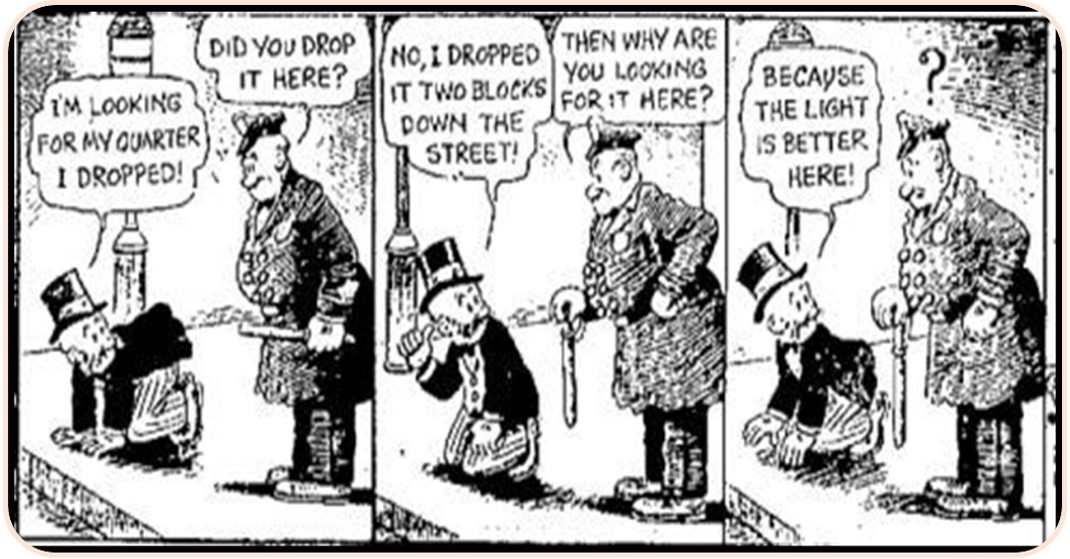
\includegraphics[width=\linewidth]{images/streetlight.jpeg}
  \end{center}
\end{column}
\end{columns}
  
\end{frame}

\begin{frame}{Better LATE than never}
  \begin{columns}[T] % align columns
    \begin{column}{0.9\textwidth}
      \begin{wideitemize}
      \item A well-identified design gives us a real set of facts
        \begin{itemize}
        \item We can debate the merits of each design, but
          establishes a gold standard
        \end{itemize}
      \item Concern is that IV for settings of interest is impossible
        \begin{itemize}
        \item Evidence suggests this is not true. Creative researchers
          have found many good examples
        \item Innovations in structural methods have incorporated
          credible designs into structural models (e.g. sufficient statistics)
        \end{itemize}
      \item Even if there are not experiments design for the
        counterfactual of interest, an internally valid estimate can
        give important grounding for a structural model that attempts
        to extrapolate
      \item Key point: using \emph{poorly} identified estimates is \textbf{not better}
        \begin{itemize}
        \item No clarity on what is causal
        \item The LATE literature is useful because it highlights \emph{what is knowable}
        \end{itemize}
      \end{wideitemize}
\end{column}
\begin{column}{0.5\textwidth}
\end{column}
\end{columns}
\end{frame}

\begin{frame}{A visual for compliers / non-compliers}
  \begin{center}
    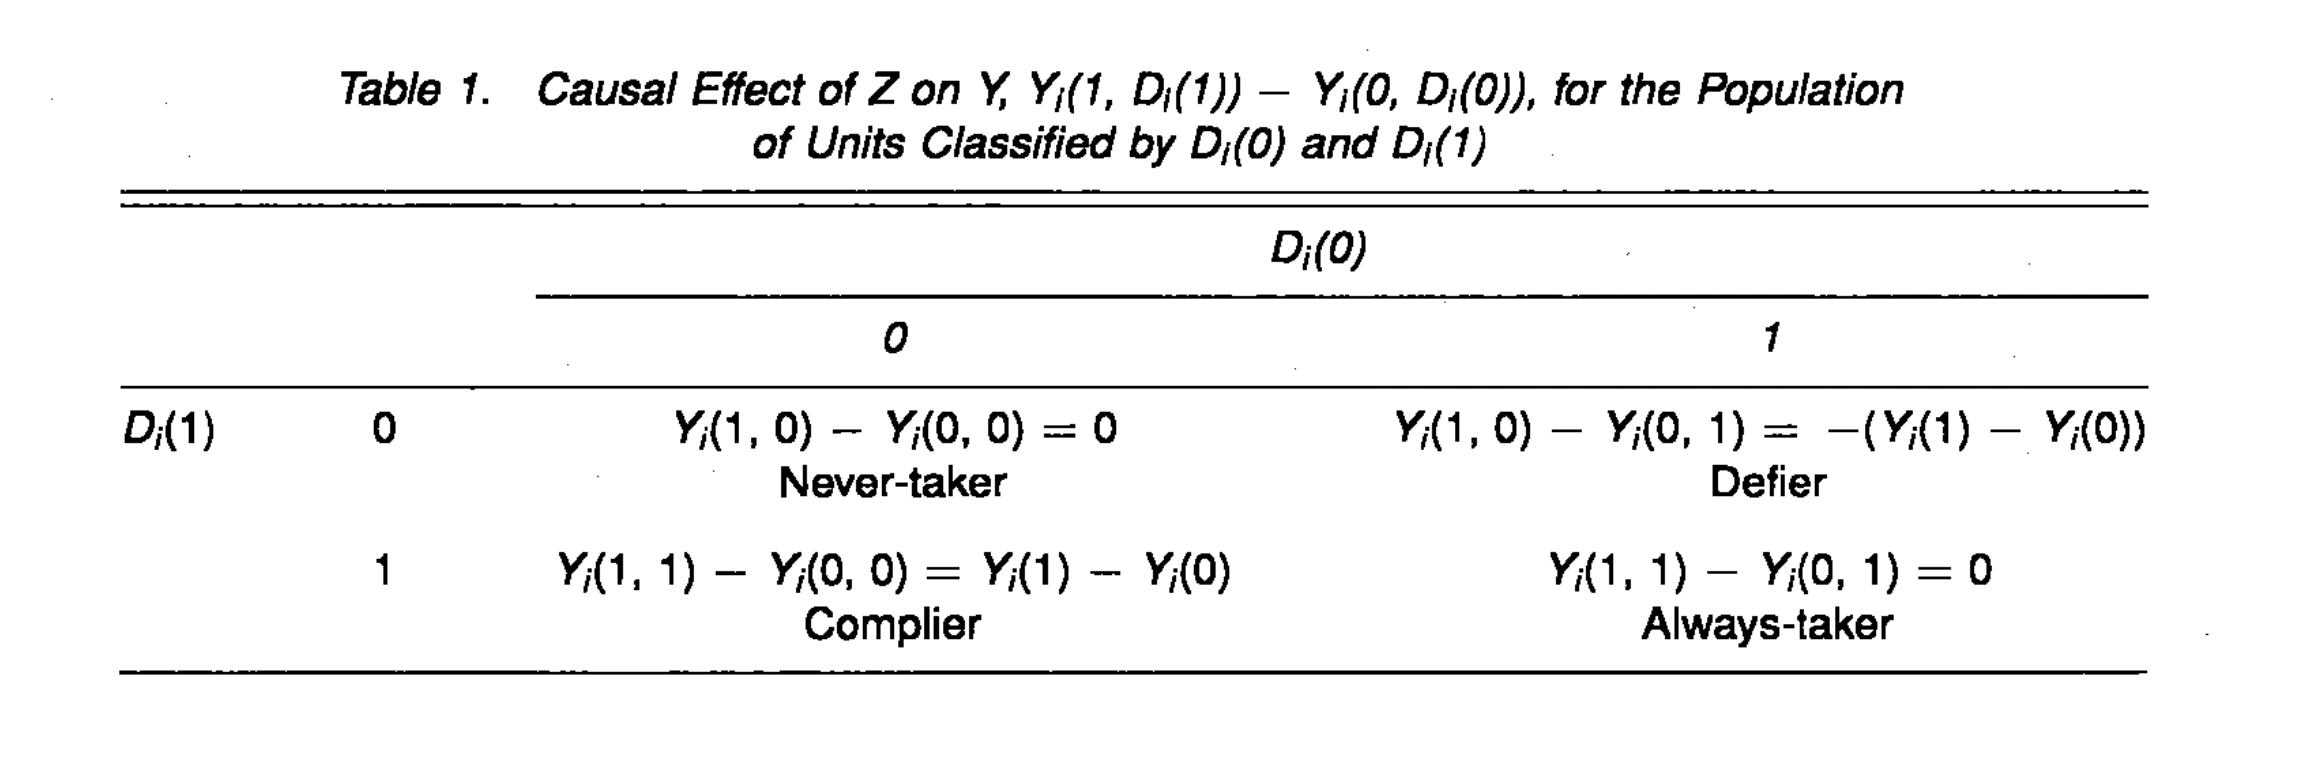
\includegraphics[width=\linewidth]{images/complier_table.png}
  \end{center}
\end{frame}

\begin{frame}{How monotonicity can fail}
  \begin{columns}[T] % align columns
    \begin{column}{0.7\textwidth}
      \begin{wideitemize}
      \item Three examples of possible failure (from de Chaisemartin
        (2017)):
        \begin{enumerate}
        \item<1-> Examiner designs: Imagine you have two judges who
          decide guilty/not guilty, and you randomly assign them. If
          monotonicity means that one judge is always stricter (for
          every person), then monotonicity holds. However, easy to
          envision failures of this (e.g. strictness on different
          crimes, different types of people)
        \item<2-> Sibling-sex composition: Angrist Evan (1998) uses
          two siblings of same sex as instrument for third child, b/c
          more likely to have a third child. But, some families may
          want two boys, vs. two girls. Same sex composition could
          generate defiers
        \item<3-> Encouragement designs may backfire if the nudge is
          too heavy-handed (Duflo and Saez (2003))
        \end{enumerate}
      \end{wideitemize}
\end{column}
\begin{column}{0.3\textwidth}
  \vspace{50pt}
  \begin{center}
  $P(z) > P(z')$\\
  vs.\\
  $D_{i}(z) \geq D_{i}(z') \forall i$
  \end{center}
\end{column}
\end{columns}

\end{frame}

\begin{frame}{Avoiding monotonicity assumption}
  \begin{wideitemize}
  \item There are a papers that attempt to characterize alternative
    assumptions (instead of monotonicity)
  \item These may work better for your particular application! See, e.g.,
    \begin{itemize}
    \item de Chaisemartin ``Tolerating defiers'' (2017)
    \item Frandsen et al. ``Judging Judge Fixed Effects'' (2019)
    \end{itemize}
  \item In the end, however, the problem is that defiers create a
    fundamental mismeasurement problem
    \begin{itemize}
    \item Any solution will attempt to alleviate this by adding extra assumptions
    \item These solutions need to be situational!
    \end{itemize}
    
  \end{wideitemize}
  
\end{frame}

\begin{frame}{IV is a useful tool for estimating causal effects in many settings}
  \begin{wideitemize}
  \item Note that IV is simply a tool for evaluating a causal impact using an instrument
  \item An example: imagine we use diff-in-diff to induce random
    variation in a policy. This can be combined with IV to construct a causal estimate:
    \begin{align}
      Y_{i} &= \alpha_{i} + \gamma_{t} + D_{it}\beta + \epsilon_{it}\\
      D_{it} &= \alpha_{i} + \gamma_{t} + Z_{it}\beta + \epsilon_{it}\\      
    \end{align}
  \item The same issues apply for both DinD and IV, but can be a
    powerful way to convert a DinD evaluation of a policy into a
    structural parameter of interest
    \begin{itemize}
    \item Need exclusion to hold, and monotonicity as well, if there
      are heterogeneous effects
    \item See discussion in ``Fuzzy difference-in-differences'' by de
      Chaisemartin and d'Haultfoeuille and ``Interpreting Instrumented
      Difference-in-Differences'' by Hudson, Hull and Liebersohn
    \end{itemize}
  \item The ``fuzzy'' label will come again with regression
    discontinuity
  \end{wideitemize}
\end{frame}

\begin{frame}{Understanding compliers}
  \begin{columns}[T] % align columns
    \begin{column}{0.7\textwidth}
      \begin{wideitemize}
      \item Under the LATE assumptions, we can know a decent amount about the compliers.
      \item First, if $D_{i}$ is binary, the difference in propensity scores (first stage) is exactly the complier share:
        \begin{equation*}
          Pr(D_{i}(1) > D_{i}(0)) = E(D_{i}(1) - D_{i}(0)) = E(D_{i} | Z_{i} = 1) - E(D_{i}|Z_{i}=0)
        \end{equation*}
      \item We can even know the share treated, using Bayes' rule:
        \begin{align*}
          Pr(D_{i}(1) > D_{i}(0) | D_{i} = 1) &= \frac{P(D_{i} = 1 | D_{i}(1) > D_{i}(0)) \times Pr(D_{i}(1) > D_{i}(0))}{Pr(D_{i} = 1)}\\
          &=\frac{P(Z_{i} = 1) \times Pr(D_{i}(1) > D_{i}(0))}{Pr(D_{i} = 1)}
        \end{align*}
      \item This identifies the share of compliers
      \end{wideitemize}
\end{column}
\begin{column}{0.3\textwidth}
\end{column}
\end{columns}

  
\end{frame}

\begin{frame}{Understanding compliers}
  \begin{columns}[T] % align columns
    \begin{column}{0.7\textwidth}
      \begin{wideitemize}
      \item Second, we can actually know average characteristics of
        compliers using the same logic, if the characteristic is
        discrete.
      \item Consider $X_{i}$ binary:
        \begin{align*}
          Pr(X_{i} | D_{i}(1) > D_{i}(0)) &= \frac{P(D_{i}(1) > D_{i}(0) | X_{i}) \times Pr(X_{i})}{Pr(D_{i}(1) > D_{i}(0))}\\
          &= \frac{\left(E(D_{i} | Z_{i} = 1, X_{i}) - E(D_{i} | Z_{i} = 0, X_{i})\right) \times Pr(X_{i})}{E(D_{i} | Z_{i} = 1) - E(D_{i} | Z_{i} = 0)}
        \end{align*}
      \item Note that if we scale by $Pr(X_{i})$, we get the relative
        probability of $X_{i}$ compared to the overall pop
        \begin{itemize}
        \item Just the ratio of the first stages for each group!
        \end{itemize}
      \end{wideitemize}
\end{column}
\begin{column}{0.3\textwidth}
\end{column}
\end{columns}

  
\end{frame}

\begin{frame}{Understanding compliers}
  \begin{columns}[T] % align columns
    \begin{column}{0.9\textwidth}
      \begin{wideitemize}
      \item Finally, Abadie (2002, JASA)  shows how to construct the potential outcomes for the compliers
      \item Let $g(Y)$ be any measurable function. Then,
        \begin{align*}
         E(g(Y_{i}(1)) | D_{i}(1) > D_{i}(0))) &= \frac{E(D_{i}g(Y_{i})|Z_{i} = 1) - E(D_{i}g(Y_{i})|Z_{i} = 0)}{E(D_{i}|Z_{i} = 1) - E(D_{i}|Z_{i}=0)}\\
         E(g(Y_{i}(0)) | D_{i}(1) > D_{i}(0))) &= \frac{E((1-D_{i})g(Y_{i})|Z_{i} = 1) - E((1-D_{i})g(Y_{i})|Z_{i} = 0)}{E(1-D_{i}|Z_{i} = 1) - E(1-D_{i}|Z_{i}=0)}\\
        \end{align*}
      \item Simplest case of $g(\cdot)$ as the identity gives the means for the two marginals
      \item Can identify distributional effects by the
        dummy functions for compliers
        \begin{itemize}
        \item         $F_{1}(y) = E(1(Y_{i}(1) \leq y | D_{i}(1) > D_{i}(0))$
        \item         $F_{0}(y) = E(1(Y_{i}(0) \leq y | D_{i}(1) > D_{i}(0))$
        \end{itemize}
      \end{wideitemize}
\end{column}
\begin{column}{0.3\textwidth}
\end{column}
\end{columns}
\end{frame}

\begin{frame}{Abadie (2002) OLS distributions}
  \begin{columns}[T] % align columns
    \begin{column}{0.3\textwidth}
      \begin{wideitemize}
      \item Good reason to think veteran status affected earnings
      \item We see negligible differences in the OLS data
      \item But veteran status is not randomly assigned
      \end{wideitemize}
\end{column}
\begin{column}{0.7\textwidth}
  \begin{center}
    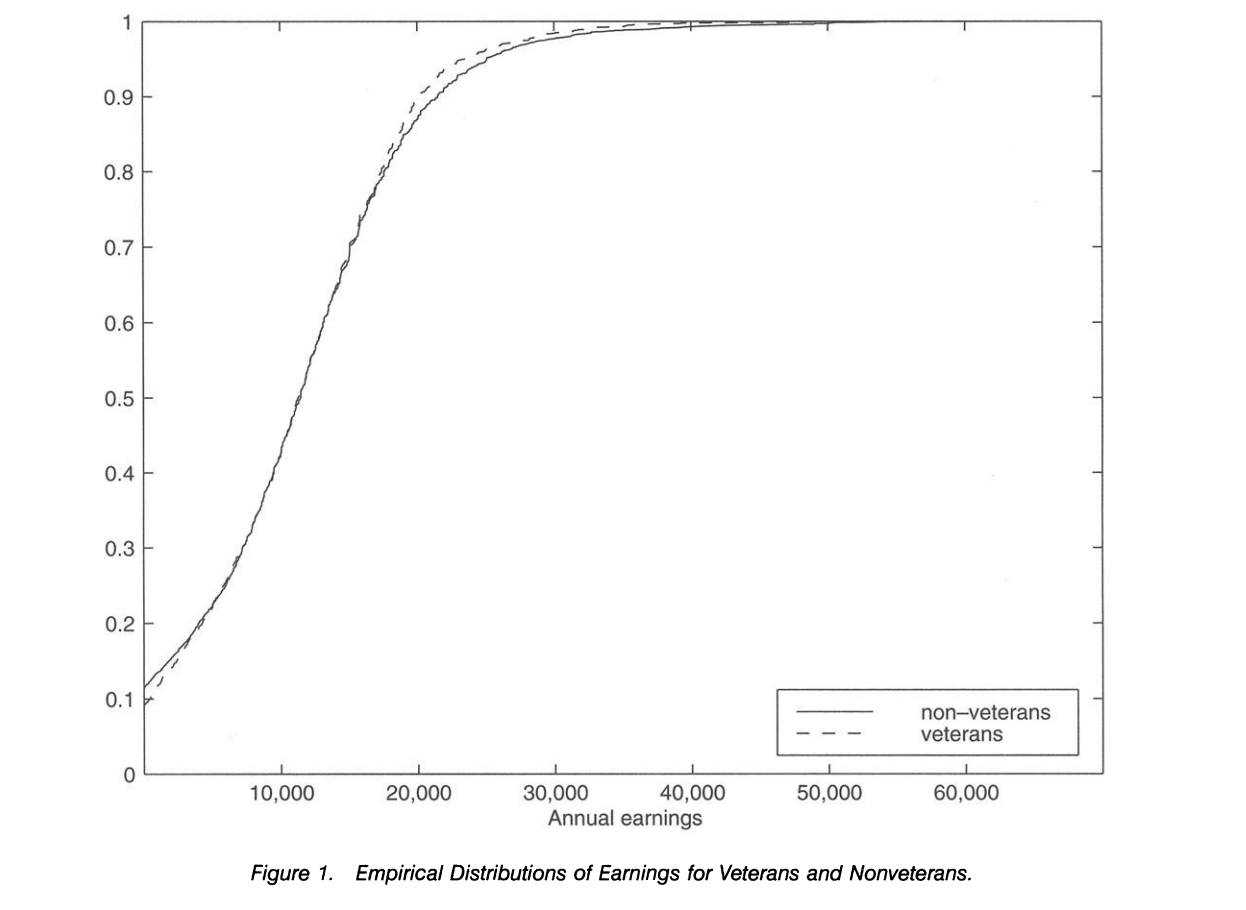
\includegraphics[width=\linewidth]{images/abadie_kappa1.png}
  \end{center}
\end{column}
\end{columns}
\end{frame}

\begin{frame}{Abadie (2002) complier distributions}
  \begin{columns}[T] % align columns
    \begin{column}{0.3\textwidth}
      \begin{wideitemize}
      \item In complier distribution, we see gap in lower part of
        distribution -- better for non-vets than vets
      \item Tests in Abadie (2002) fail to find evidence of
        differences in the distribution, however
      \end{wideitemize}
\end{column}
\begin{column}{0.7\textwidth}
  \begin{center}
    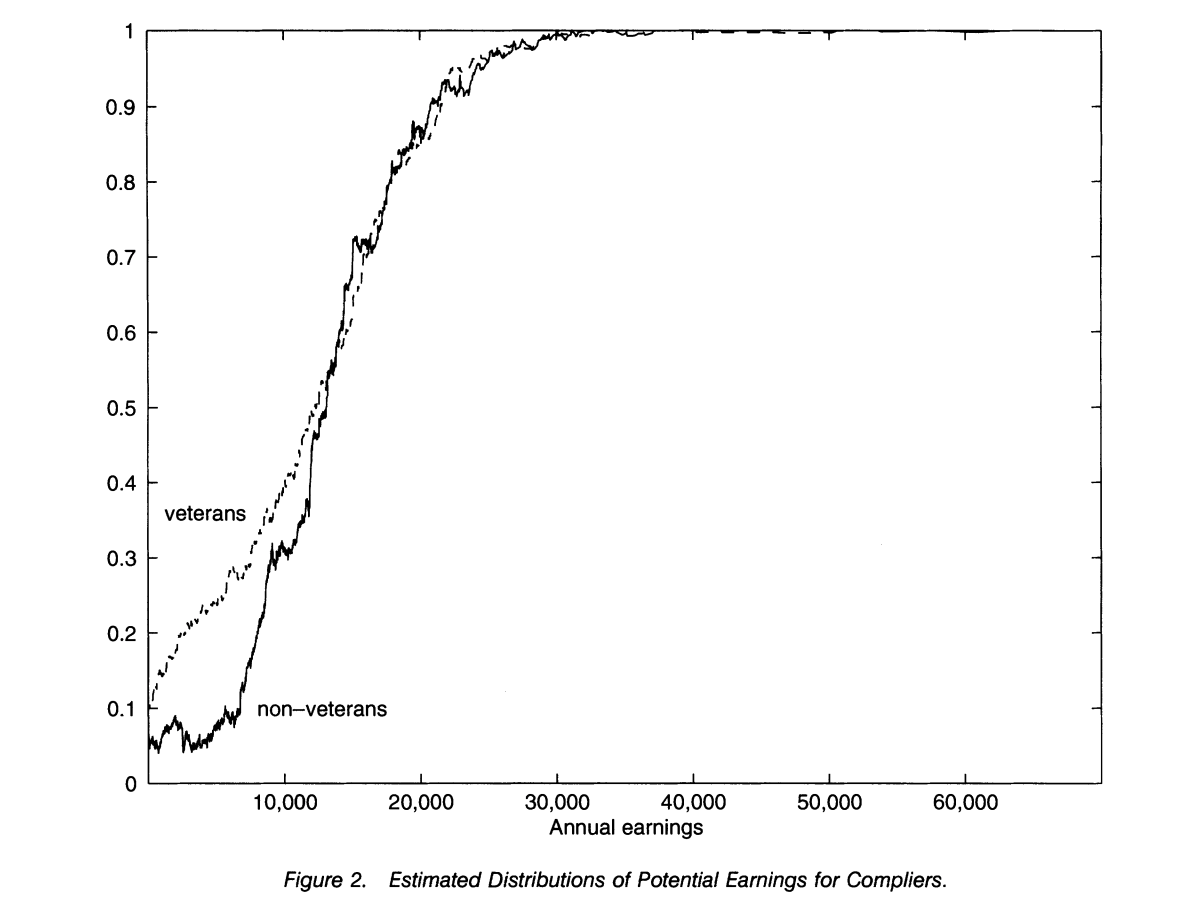
\includegraphics[width=\linewidth]{images/abadie_kappa2.png}
  \end{center}
\end{column}
\end{columns}
\end{frame}


\end{document}


\begin{frame}{Many IV and Weak IV bias}
  \begin{columns}[T] % align columns
    \begin{column}{0.9\textwidth}
  \begin{wideitemize}
  \item Now, let's pivot to estimation issues. First, a fact (that we will  explain):
    \begin{itemize}
    \item 2SLS is biased (but consistent) when you are overidentified
    \item Just-identified 2SLS estimator is not biased, but also does not have a
      finite sample mean
    \end{itemize}

  \end{wideitemize}
\end{column}
\begin{column}{0.3\textwidth}
\end{column}
\end{columns}
\end{frame}


\begin{frame}{Weak IV bias}

  PICTURE FROM Andrews, Stock and Sun
  
\end{frame}
